% ============================================================================
% Situation : equilibre d une planche (masses 12 kg et 18 kg)
% Extrait de la fiche : Barycentres et lignes de niveau (classe de 1ere D)
% Necessite \usepackage{tikz} et \usetikzlibrary{calc} (charges par le fichier principal)
% ============================================================================
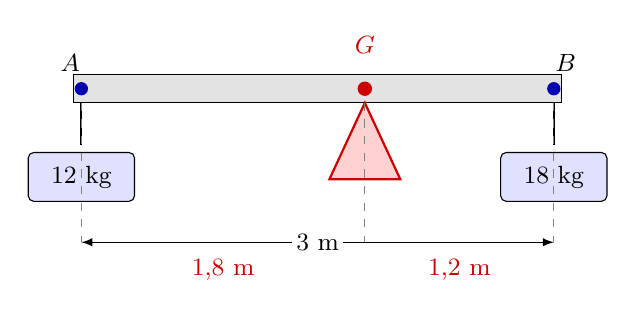
\begin{tikzpicture}[scale=1.0,>=latex]
  \draw[fill=gray!22,draw=black] (-0.1,-0.18) rectangle (6.1,0.18);
  \fill[blue!70!black] (0,0) circle (2.4pt); \fill[blue!70!black] (6,0) circle (2.4pt);
  \fill[red!80!black] (3.6,0) circle (2.6pt);
  \node[above left=-3pt,font=\small] at (0,0.2) {$A$}; \node[above right=-3pt,font=\small] at (6,0.2) {$B$};
  \node[red!80!black,font=\small] at (3.6,0.55) {$G$};
  \draw[fill=red!18,draw=red!80!black,thick] (3.6,-0.18) -- (3.15,-1.15) -- (4.05,-1.15) -- cycle;
  \draw[thick] (0,-0.18) -- (0,-0.72); \draw[thick] (6,-0.18) -- (6,-0.72);
  \node[draw,rounded corners=2pt,fill=blue!12,font=\small,minimum width=1.35cm,minimum height=0.62cm] at (0,-1.12) {12 kg};
  \node[draw,rounded corners=2pt,fill=blue!12,font=\small,minimum width=1.35cm,minimum height=0.62cm] at (6,-1.12) {18 kg};
  \draw[<->] (0,-1.95) -- (6,-1.95) node[midway,fill=white,inner sep=1.5pt,font=\small] {$3$ m};
  \draw[dashed,gray] (0,-0.18) -- (0,-1.95); \draw[dashed,gray] (6,-0.18) -- (6,-1.95);
  \draw[dashed,gray] (3.6,-0.18) -- (3.6,-1.95);
  \node[red!80!black,font=\small] at (1.8,-2.3) {$1{,}8$ m};
  \node[red!80!black,font=\small] at (4.8,-2.3) {$1{,}2$ m};
\end{tikzpicture}
